\section{Problem Setup}\label{background}

\subsection{Motivating Analysis Scenario}
Large dirty data are prevelant \cite{fortunearticle}, and we introduce an example of systematic corruption in publically available data. We present the following running example with our Dollars for Docs dataset (see Experiments, Section \ref{dfd-exp}):

\vspace{0.25em}

\noindent\textbf{Dollars for Docs. }
ProPublica has collected a dataset of corporate contributions to doctors for analysis of whether these contributions (negatively) affect research. 
The dataset has the following schema:
\begin{lstlisting}[mathescape,basicstyle={\scriptsize}]
Contribution(pi_speciality$\textrm{,}$ drug_name$\textrm{,}$ device_name$\textrm{,}$ corporation$\textrm{,}$ amount$\textrm{,}$ dispute$\textrm{,}$ status)
\end{lstlisting}

\noindent\texttt{pi\_speciality} is a textual attribute describing the speciality of the doctor recieving the contribution.

\noindent\texttt{drug\_name} is the branded name of the drug in the research study (null if not a drug).

\noindent\texttt{device\_name} is the branded name of the device in the study (null if not a device).

\noindent\texttt{amount} is a numerical attribute representing the contribution amount.

\noindent\texttt{dispute} is a boolean attribute describing whether the research was disputed.

\noindent\texttt{status} is a string label describing whether the contribution was covered under the declared research protocol. There are two statuses ``Covered" and ``Non-Covered".

\vspace{0.25em}

\noindent Using this dataset, consider the following analysis scenario.
\begin{example}
We are interested in predicting impropriety in medical research contributions, by exploring what features of a research contribution predict the \texttt{status} (i.e., whether it was not allowed by the protocol).
We featurize the textual attributes with a bag-of-words model and treat the \texttt{amount}/\texttt{dispute} attributes as numerical features.
The predictive model is a Support Vector Machine (SVM) that predicts the label $\{1,0\}$ where $1$ indicates a disallowed contribution.
\end{example}

However, this dataset is very dirty, and the systematic nature of the corruption can result in a misleading model.
On the Pro Publica website \cite{dollarsfordocs}, they list numerous types of corruption that had to be cleaned before publishing the data (see Appendix \ref{dfd-errors}).
For example, the most significant contributions were made by large companies whose names were also more often inconsistently represented in the data e.g. ``Pfizer Inc.", ``Pfizer Incorporated", ``Pfizer".
In a fraud detection scenario such as this one, the effect of systematic error can be serious.
Duplicate entity representations, could reduce the correlation between these entities and impropriety.

\vspace{0.25em}

\noindent\textbf{Cleaning With a Budget: }  Let us suppose our analyst wants evaluate whether the problems affect her model, and she wants to do this without having to manually validate every record. 
The first solution to this problem is to clean a sample of data, write this sample back, and then retrain the model on the partially cleaned data.
However, this solution can give unreliable results since we are mixing dirty and clean data.
In Figure \ref{update-arch1}, we illustrate the dangers of this approach on a very simple dirty dataset and model.
Suppose, we are trying to find a best fit line for two variables. 
One of the variables is systematically corrupted with a translation in the x-axis (Figure \ref{update-arch1}a).
We mark the dirty data in brown and the clean data in orange, and show their respective best fit lines in blue.
If we clean two of the data points (Figure \ref{update-arch1}b), and then find the best fit line, the partially cleaned model is dramatically incorrect.
This is a well-known phenomenon called Simpsons paradox, where mixtures of different populations of data can result in spurious relationships \cite{simpson1951interpretation}.
The result is surprising, namely, Machine Learning on partially cleaned data can lead to misleading results.

The next solution is avoiding the dirty data altogether.
She can take a sample of data, apply data cleaning, and train a model only on that sample of data.
This is similar to SampleClean \cite{wang1999sample}; proposed to approximate the results to aggregate queries by applying them to a clean sample of data.
Machine Learning models are highly senstive to sample size when high dimensional.
The result is that the models will not be useful (i.e., cannot accurately predict test data) when the sample size is too small (Figure \ref{update-arch1}c).

\begin{figure}[ht!]
\centering
 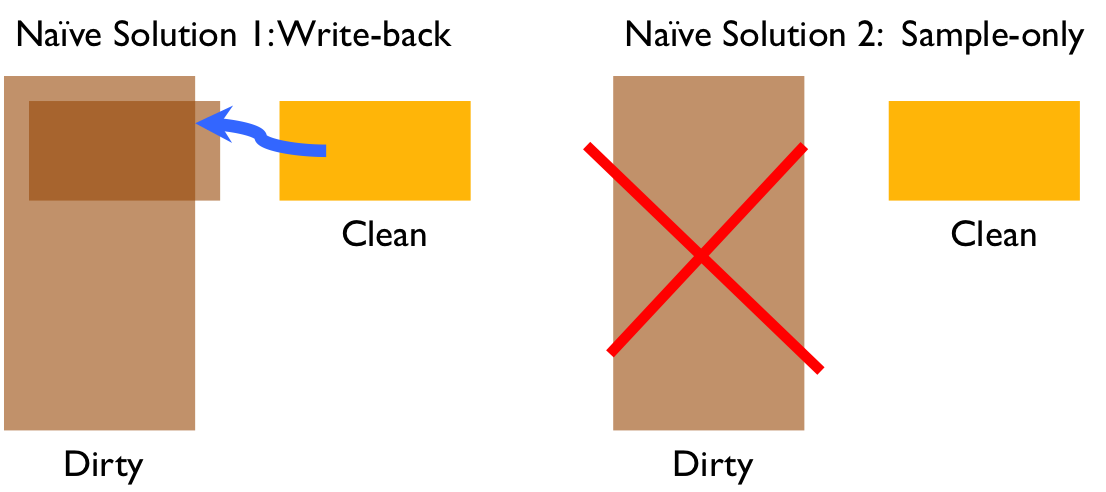
\includegraphics[width=\columnwidth]{figs/update-arch.png}
 \caption{(a) We present a dataset with a systematic corruption (translation) in one variable where the dirty data is in brown and the clean data is in yellow. If we draw the best fit line (i.e., linear regression), we see that the systematic corruption affects the line.
 (b) However, after cleaning two data points, applying the same model to partially clean data results in a dramatically incorrect answer.
(c) Likewise, small sample sizes can result in similarly incorrect models. \label{update-arch1}}
\end{figure}

\sys avoids both pitfalls, Simpsons's paradox and sample size dependence.
In Section \ref{model-update}, we show how we do this with iterative gradient steps (i.e., incrementally moving the line based on the clean data).
This takes advantage of the dirty data as well as the clean data, but still have provable properties about the intermediate results.
In Figure \ref{sys-arch2}, we illustrate our ideal tradeoff space of sampling and data cleaning.
At two extremes we have no cleaning (just using the dirty data) and full cleaning.
\sys is optimized for convergence for smaller sample sizes than a uniform sampling approach.

\begin{figure}[t]
\centering
 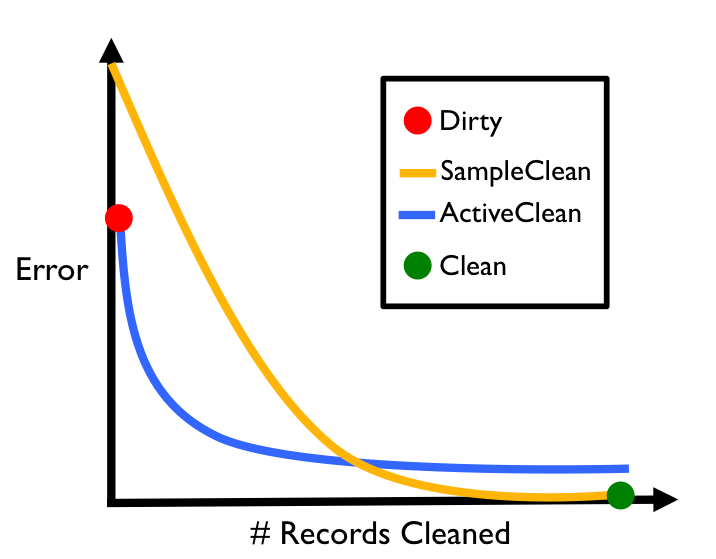
\includegraphics[width=0.5\columnwidth]{figs/arch2.png}
 \caption{Our goal with \sys is designed to converge to an accurate model with fewer cleaned records than a uniform sampling approach (SampleClean). \label{sys-arch2}}\vspace{-1em}
\end{figure}

\iffalse

We design \sys to make greater progress at these small sample sizes using the dirty model as an initialization.
Doing so is not trivial since it requires analysis of both the Machine Learning model and the data cleaning operations.
Data may look unimportant to a dirty model but when cleaned are very important.
Also, data cleaning and model training can happen at very different time scales, we have to carefully budget our effort to ensure that any optimizations actually address rate-determining steps in the workflow.
Finally, in this line of work, the tradeoff space is enormous, and we have to carefully pick a design point and tailor our optimizations to this preferred regime.
\fi

\subsection{Preliminaries}
\iffalse
There have been a few proposals of tighter integration of data cleaning and analytics.
In SampleClean \cite{wang1999sample}, the authors formalize the analytics in terms of a SQL aggregate query.
Bergman et al. explore the problem of query-oriented data cleaning \cite{bergman2015query}, where a conjunctive query (CQ) guides which records are to be cleaned.
SQL and CQ formalize a declarative problem specification in database research.
In a loose analogy to the declative queries in databases, loss functions in serve the same purpose in ERM.
\fi

We focus on a class of Supervised Learning problems called Empirical Risk Minimization (ERM) (see Friedman, Hastie, and Tibshirani \cite{friedman2001elements} for an introduction).
In ERM, the goal is to learn a set of model \emph{parameters} $\theta$ from training examples.
We start with a set of training examples $\{(x_{i},y_{i})\}_{i=1}^{N}$
on which we minimize a loss function $\phi$ (a penalty for getting the prediction wrong) at each point parametrized by $\theta$.
A very important class of problems is when the loss function is convex in $\theta$.
Convex problems are amenable to a variety of different optimization methodologies
and have strong theoretical guarantees on convergence rates.
This class of problems includes all generalized linear models (including linear and logistic regression), and all variants of support vector machines.
Formally,
\[
 \theta^{*}=\arg\min_{\theta}\sum_{i=1}^{N}\phi(x_{i},y_{i},\theta)
\]
For example, in a linear regression $\phi$ is:
\[
\phi(x_{i},y_{i},\theta) = \|\theta^Tx_{i} - y_i \|_2^2
\]
Typically, a \emph{regularization} term $r(\theta)$ is added to this problem.
$r(\theta)$ penalizes high or low values of feature weights in $\theta$ to avoid overfitting to noise in the training examples.
\[
 \theta^{*}=\arg\min_{\theta}\sum_{i=1}^{N}\phi(x_{i},y_{i},\theta) + r(\theta)
\]
For example, a popular variant of linear regression is called LASSO which is:
\[
 \theta^{*}=\arg\min_{\theta}\sum_{i=1}^{N}\|\theta^Tx_{i} - y_i \|_2^2 + \lambda \cdot \|\theta\|_1
\]
By applying the L1 regularization term, if one of the features is particularly noisy, and does not add predictive value, it will get excluded.
The loss function specifies a problem independent of the optimization used to calculate the optimal parameter $\theta^{*}$.

\subsubsection{Types of Errors}
When discussing ``errors" in Machine Learning models, we refer to the following metrics:

\vspace{0.25em}

\noindent\textbf{Model Error. } Let $\theta$ be the model trained on the dirty data, and let $\theta^*$ be the model trained on the same data if it were cleaned. Then the model error is defined as $\|\theta - \theta^*\|$.

\vspace{0.25em}

\noindent\textbf{Testing Error. } Let $\theta$ be the model trained on the dirty data, and let $\theta^*$ be the model trained on the same data if it were cleaned. Let $T(\theta)$ be the out-of-sample testing error when the dirty model is applied to the clean data, and $T(\theta^*)$ be the test error when the clean model is applied to the clean data. The testing error is defined as $T(\theta^*) - T(\theta)$

\vspace{0.5em}

\noindent The \emph{error} in the model and in testing is caused by two underlying problems:

\vspace{0.25em}

\noindent\textbf{Data Error. } Error caused by dirtiness.

\vspace{0.25em}

\noindent\textbf{Sampling Error. } Error introduced by sampling i.e., the difference between a model trained on $p\%$ of the data and $100\%$ of the data.

\vspace{0.25em}

In this paper, when we use the term \emph{error}, we are refering to \textbf{model error}.
We will be explicit when we are using the word error to describe problems regarding dirtiness in the underlying data (e.g. ``data corruption").

\subsection{\sys Problem}
The basic question that we explore in this work is how to update a model trained on dirty data with data cleaning. Formally,

\begin{problem}[ActiveClean Problem]\label{activeclean}\sloppy
Let $R$ be a dirty relation and each row $r \in R$ is 
turned into a feature vector and label tuple $F(r) \mapsto (x,y)$.
We are given a convex regularized loss model parametrized
by $\theta$ trained on the set of features and labels $\{(x,y)\}$.
The user specifies a data repair step which cleans a record 
$C(r) \mapsto r_{clean}$.
Optionally, the user can provide a set of dirty data detection conditions that select 
a set of candidate dirty data $R_{dirty}$.
With a budget of applying cleaning i.e., $C(\cdot)$, only k times, return an estimate $\hat{\theta}$ of the clean model.
\end{problem}

Our goal is to use information from the model to inform data cleaning on samples, and use the information from clean samples to update the model.
The tight feedback loop between model training and data cleaning poses several new algorithmic challenges. 
If we are not careful about how we update the model, we can end up with the Simpsons paradox problem described before.
Data cleaning and model training happen at very different time scales, we have to carefully budget our effort to ensure that optimizations address rate-determining steps in the workflow.

This framework is optimized around problems with expensive data cleaning.
As the complexity of dirtiness increases, so does the amount of computation and human-effort needed to resolve them.
The consequence is that automated repair is either not scalable or relies on greedy repairs that can be unreliable.
Increasingly, human effort is seen as valuable in data cleaning \cite{park2014crowdfill, wang2012crowder, gokhale2014corleone, wang1999sample}.
When humans are involved, per record latencies for data repair are orders of magnitude larger than the CPU time needed for model training.
We can compare recent results in data cleaning to a model training framework like CoCoA implemented on Spark \cite{jaggi2014communication}.
Per record, BigDansing, a highly optimized automated Spark-based data cleaning system is 15.5x slower than CoCoA\footnote{For CoCoA to reach a precision of 1e-3}.
Crowd based techiques like CrowdFill \cite{park2014crowdfill} and CrowdER \cite{wang2012crowder} are over 100,000x slower per record.

\noindent Here is an example application of \sys with our running example:
\begin{example}
The analyst first trains her SVM model on the dirty data ignoring the effects of the errors returning a model $\theta^{(d)}$.
She decides that she has a budget of cleaning $100$ records, and decides to clean the 100 records in batches of 10 (set based on how fast she can clean the data, and how often she wants to see an updated result).
She initializes \sys with $\theta^{(d)}$.
\sys samples an intial batch of 10 records.
She manually cleans those records by using the medical record source data.
After each batch, the model is updated with the most recent cleaning results $\theta^{(t)}$.
The model improves after each iteration.
After $t=10$ of cleaning, the analyst has an accurate model trained with 100 cleaned records but still utilizes the entire dirty data.
\end{example}

\iffalse

\subsection{Two perspectives on error}
When faced with such errors there are two contrasting perspectives from the Machine Learning and the Database communities.

\vspace{0.5em}

\noindent\textbf{Existing Database Literature. } 
Traditionally, cleaning is agnostic to the queries and analysis that happens downstream. 
This perspective breaks down when cleaning is so expensive that we can only clean a small number of records.
Ideally, we should clean the records that are most valuable to the downstream analysis.

\vspace{0.5em}

\noindent\textbf{Existing  Machine Learning Literature. } The Machine Learning community has focused on
designing models that are robust to outliers (i.e., values far away from the typical value)
For example, in the case of linear regression, we can change the $L_2$ norm to an $L_1$ norm to mitigate the effect of outliers:
\[
\phi(x_{i}^T\theta,y_{i}) = \|\theta^Tx_{i} - y_i \|_1
\]
The quadratic L2 loss implies that examples that deviate far from the typical example are quadratically penalized as opposed to linearly penalized with the L1 loss.
There is a natural tradeoff between robustness and efficiency.
The more robust a technique is, the less efficient it will be (i.e., estimate variance for a fixed number of training examples).
Robust techniques are best suited for random errors that look significantly different the rest of the examples.
When errors are systematic, the Machine Learning answer has been to design features in such a way that they are robust to some systematic bias.
For example, in image processing, scale-invariant feature transforms (SIFT) are widely applied that allow for image models invariant to pose or scaling issues.

\vspace{0.5em}

\noindent\textbf{The \sys Contribution. } We try to bring two perspectives together in this work to address the problem of expensive to clean systematic errors, namely the Database idea of data cleaning and the Machine Learning formalization of empirical risk minimization.
Some errors require expensive cleaning procedures, increasingly using the crowd, and we joint have a time budget on cleaning and analysis.
\sys prioritizes cleaning with respect to an estimated impact on the clean model.



\subsection{SampleClean Project}

Traditionally, data cleaning has explored expensive, up-front cleaning of entire datasets for increased query accuracy.
We proposed the SampleClean problem, in which an analyst cleans a small sample of data, and then estimates the result to an aggregate query e.g., \sumfunc, \countfunc, or \avgfunc.
The main insight from the SampleClean project is that highly accurate answers for aggregate queries does not require cleaning the full dataset.
Generalizing this insight, there is a deep relationship between the application (i.e., the query) and how an analyst should budget their effort in data cleaning.
In fact, \avgfunc and \sumfunc queries are a special case of the convex loss minimization discussed in the previous section:
\[
\phi = (x_{i} - \theta)^2
\]

We then extended the SampleClean work to study cleaning Materialized Views \cite{technicalReport}.
Suppose base data is updated with insertions, deletions, or updates, we explored how we could efficiently propagate
changes to a sample of the view instead of the full view.
Subsequent queries on the view could be answered approximate.

The SampleClean problem inspired an eponymous system that implements sampling, data cleaning, and approximate query processing on the Apache Spark stack \cite{sampleclean}.
Also included in the Apache Spark stack are Machine Learning libraries including MLlib \cite{mllib} and GraphX \cite{graphx}.
The in-memory architecture of the Apache Spark stack allows for increasingly interactive analysis \cite{AgarwalMPMMS13, armbrust2015spark}.
Analysts can prototype data processing workflows on samples to evaluate performance before running expensive batch processing jobs on entire datasets.
With data cleaning and machine learning libraries in the same software ecosystem, we see a new opportunity for joint optimization for interactive model building.



\subsection{Stochastic Gradient Descent}
Sampling is a natural part of any Machine Learning workflow, as stochastic optimization is widely used to fit model parameters.
The problems described in the previous subsections are often trained using a technique called Stochastic Gradient Descent (SGD) or one of its variants.
The basic idea of SGD is to draw a data point at random, calculate the gradient at that point, and then update a current best estimate with that gradient.
\[
\theta^{(t+1)}\leftarrow\theta^{(t)}-\gamma\nabla\phi(x_{i}^T\theta,y_{i})
\]
 SGD can also be applied in a ``mini-batch" mode, where we draw a subset of data $S^{(t)}$ at random and update with the average gradient.
 \[
 \theta^{(t+1)}\leftarrow\theta^{(t)}-\frac{\gamma}{\|S^{(t)}\|}\sum_{i\in S^{(t)}}\nabla\phi(x_{i}^T\theta,y_{i})
 \]

We can use this workflow for designing an anytime data cleaning methodology.
As data is sampled, we can clean the samples.
The analyst then can stop at anytime and use the best model at that instant.
SGD and its variants are well-studied and there are lower-bounds on the convergence rates using these techniques. 
Recently, a number of works have explored non-uniform sampling distributions for stochastic optimization \cite{zhao2014stochastic, qu2014randomized}.
The main insight is that non-uniform distributions may on average estimate the gradient accurately.
In this work, we explore how to design such a non-uniform distribution for iterative data cleaning.

\fi


 